\section{Wykorzystanie CO$_2$}

\begin{columnframe}{CCU: Carbon Capture and Utilization - Wykorzystanie CO$_2$}
    \begin{column}{0.5\textwidth}
        \begin{figure}
            \centering
            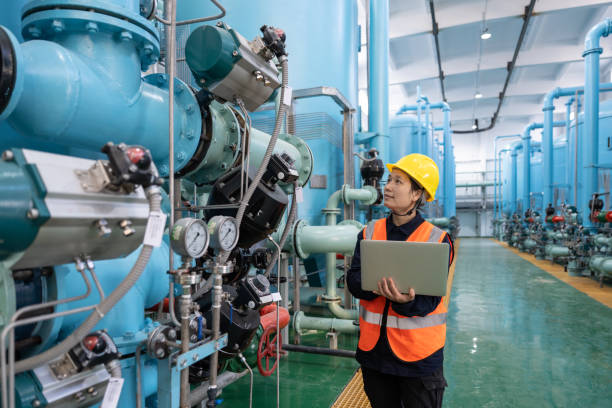
\includegraphics[width=0.8\textwidth, frame]{images/chemical_engineering_stock_image.jpg}
        \end{figure}
    \end{column}
    \begin{column}{0.5\textwidth}
        \begin{itemize}
            \item Wychwytane CO$_2$ może być wykorzystane w przemyśle chemicznym.
            \item Pozwala to na pośrednią redukcję emisji CO$_2$: inaczej trzeba byłoby pozyskiwać je z innych źródeł
        \end{itemize}
    \end{column}
\end{columnframe}

\begin{columnframe}{EOR (Enhanced Oil Recovery)}
    \begin{column}{0.5\textwidth}
        \begin{itemize}
            \item w przemyśle naftowym CO$_2$ jest wykorzystywane do zwiększenia wydobycia ropy.
            \item Wstrzykiwanie CO$_2$ do złoża zwiększa ciśnienie i zmniejsza gęstość, co ułatwia wydobycie .
        \end{itemize}
    \end{column}
    \begin{column}{0.5\textwidth}
        \begin{figure}
            \centering
            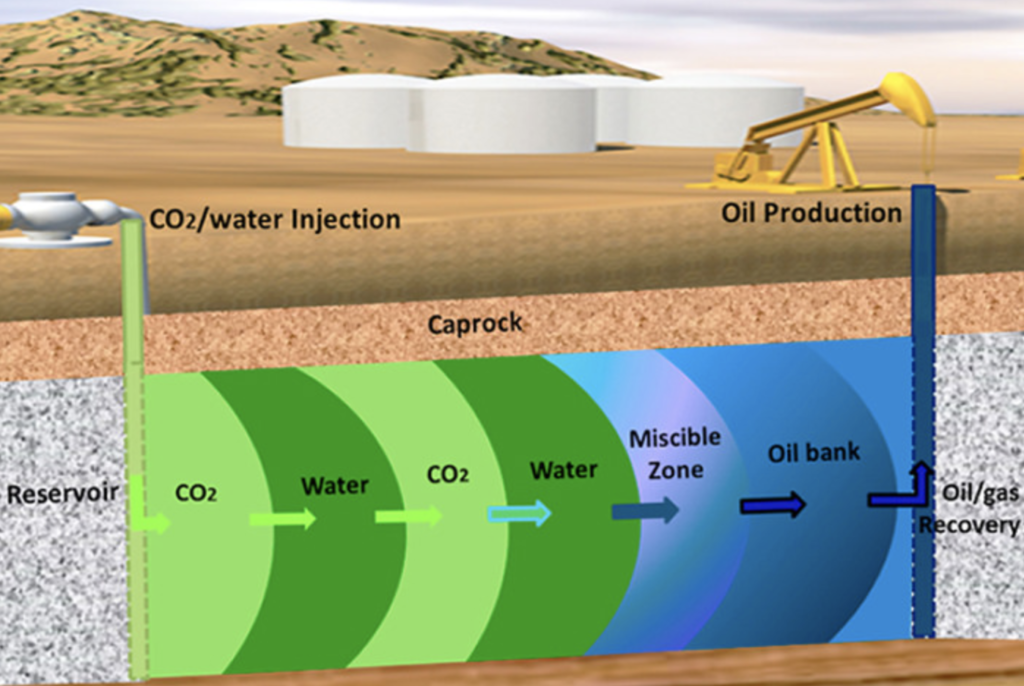
\includegraphics[width=0.8\textwidth, frame]{images/enhanced_oil_recovery.png}
        \end{figure}
    \end{column}
\end{columnframe}

\begin{columnframe}{Jedzenie}
    \begin{column}{0.5\textwidth}
        \begin{figure}
            \centering
            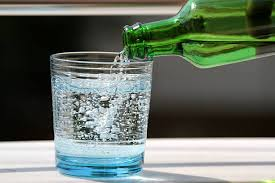
\includegraphics[width=0.9\textwidth, frame]{images/carbonated_water_stock_image.jpg}
        \end{figure}
    \end{column}
    \begin{column}{0.5\textwidth}
        \begin{itemize}
            \item CO$_2$ może być wykorzystane w przemyśle spożywczym do produkcji napojów gazowanych.
            \item Jest także wykorzystywane do zwiększenia wydajności upraw roślin (kwas węglowy).
        \end{itemize}
    \end{column}
\end{columnframe}

\begin{columnframe}{Hodowanie glonów}
    \begin{column}{0.5\textwidth}
        \begin{itemize}
            \item Algi są w stanie przetwarzać CO$_2$ na tlen i biomasy.
        \end{itemize}
    \end{column}
    \begin{column}{0.5\textwidth}
        \begin{figure}
            \centering
            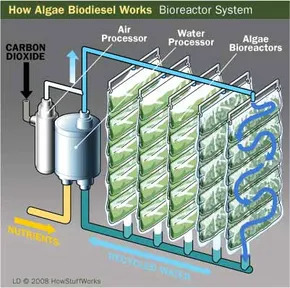
\includegraphics[width=0.9\textwidth, frame]{images/algae_biodiesel.jpg}
        \end{figure}
    \end{column}
\end{columnframe}

\begin{columnframe}{Produkcja plastiku}
    \begin{column}{0.5\textwidth}
        \begin{figure}
            \centering
            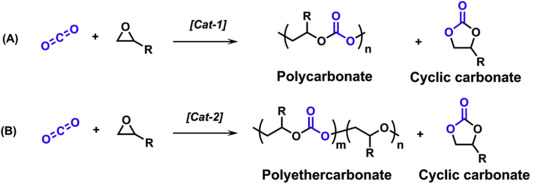
\includegraphics[width=0.95\textwidth, frame]{images/plastic_from_co2.jpg}
        \end{figure}
    \end{column}
    \begin{column}{0.5\textwidth}
        \begin{itemize}
            \item CO$_2$ może być wykorzystane do produkcji polimerów.
        \end{itemize}
    \end{column}
\end{columnframe}

\begin{columnframe}{Metanizacja (Sabatier reaction)}
    \begin{column}{0.5\textwidth}
        \begin{itemize}
            \item CO$_2$ pochodzące z powietrza lub z procesów przemysłowych może być przekształcone w metan, który może być wykorzystany jako paliwo.
            \item Ten proces wymaga wysokiej temperatury (około 300-400$^\circ$C)
        \end{itemize}
    \end{column}
    \begin{column}{0.5\textwidth}
        \[
            \ch{CO2} + 2\ch{H2O} \rightarrow \ch{CH4} + 2\ch{O2}
        \]
    \end{column}
\end{columnframe}

\begin{columnframe}{Biometan jako paliwo}
    \begin{column}{0.5\textwidth}
        \begin{figure}
            \centering
            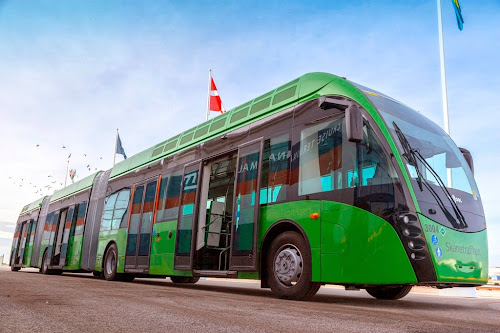
\includegraphics[width=0.9\textwidth, frame]{images/Biomethane_bus_malmo.jpg}
            \caption{Autobus zasilany biometanem w Malmo, Szwecja}
        \end{figure}
    \end{column}
    \begin{column}{0.5\textwidth}
        \begin{itemize}
            \item Biometan ma wysoki stosunek energii do masy (niższy niż benzyna, wyższy niż wodór)
            \item Można wykorzystywać je w silnikach spalinowych
        \end{itemize}
    \end{column}
\end{columnframe}

\begin{columnframe}{Rakieta na metan: Raptor 3}
    \begin{column}{0.5\textwidth}
        \begin{itemize}
            \item Rakieta Starship, która ma być używana do lotów na Marsa, będzie zasilana metanem.
            \item Metan przy spalaniu w silnikach rakietowych daje mniejsze ilości zanieczyszczeń niż tradycyjne paliwa rakietowe.
        \end{itemize}
    \end{column}
    \begin{column}{0.5\textwidth}
        \begin{figure}
            \centering
            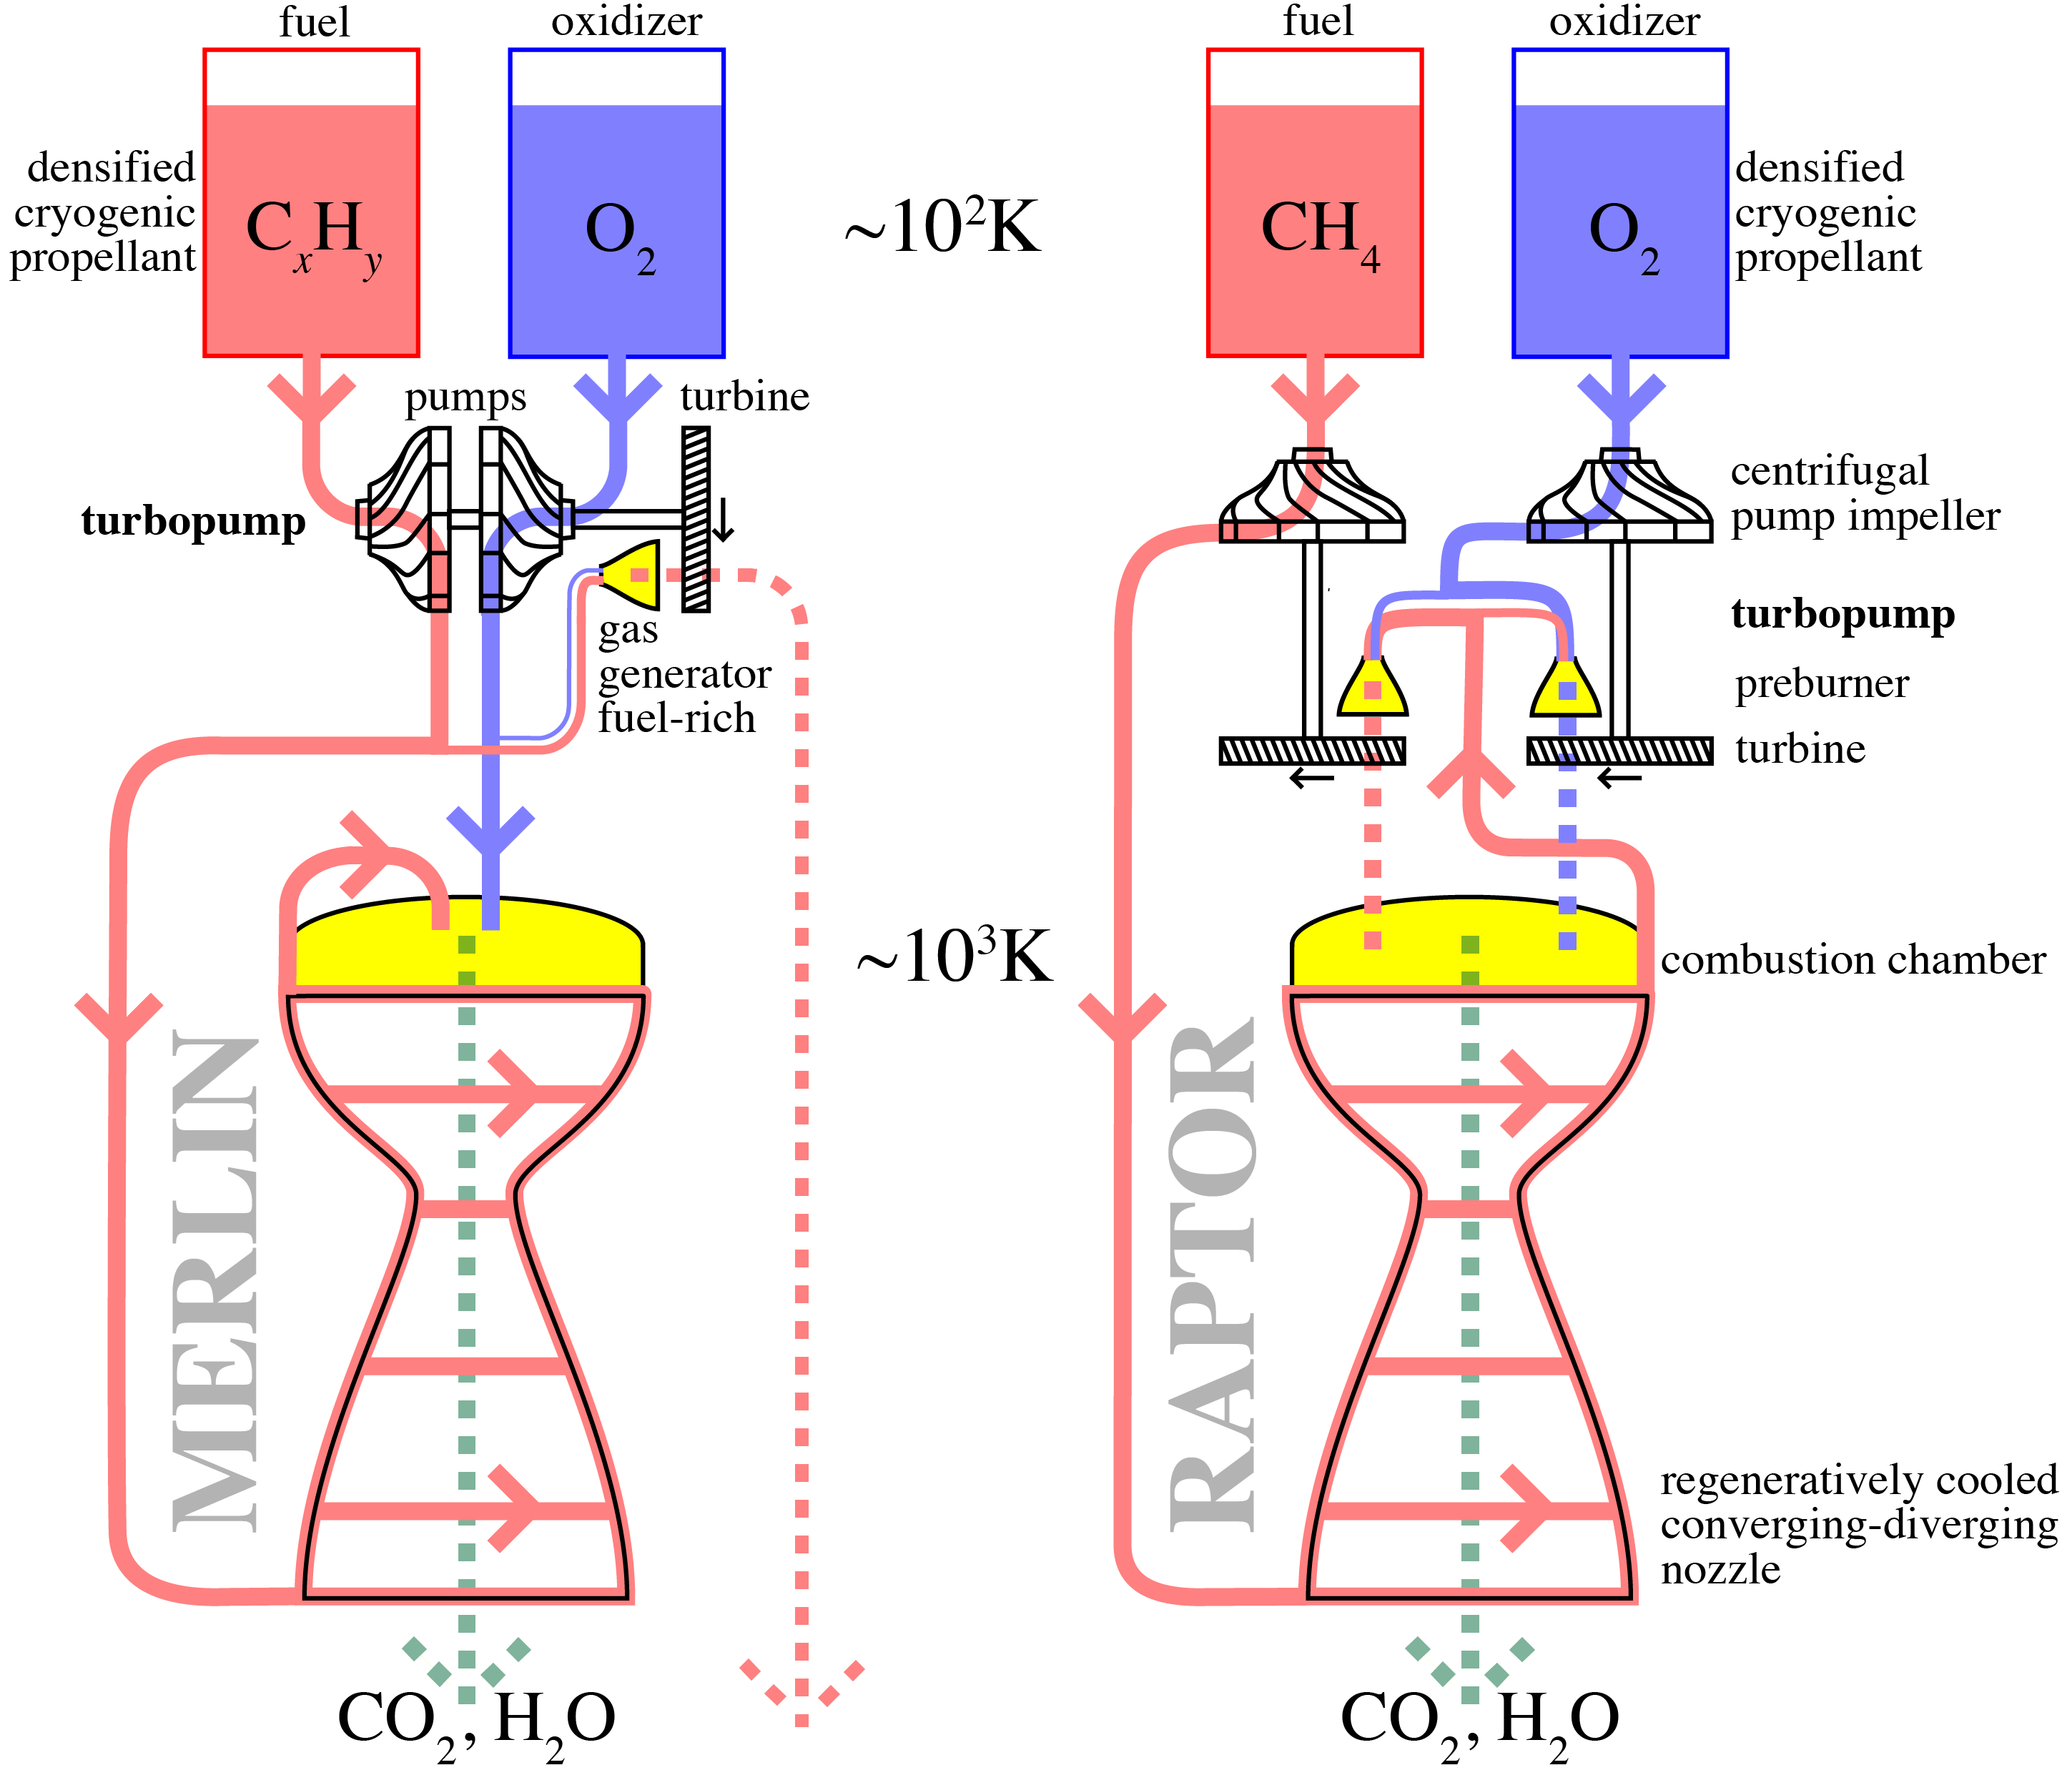
\includegraphics[width=0.9\textwidth, frame]{images/Raptor3_Merlin_comparison.png}
            \caption{SpaceX Raptor 3}
        \end{figure}
    \end{column}
\end{columnframe}

